\documentclass[a4paper,12pt]{article}
\usepackage{amsfonts}
\usepackage{amssymb}
\usepackage{latexsym}
\usepackage{amsmath}
\usepackage{amsthm}
\usepackage{graphicx}
\usepackage{indentfirst}
\usepackage[polish]{babel}
\usepackage[T1]{fontenc}
\usepackage[utf8]{inputenc}
\usepackage{setspace}
\usepackage{array}
\usepackage{multirow}
\usepackage{geometry}
\usepackage{float}
\usepackage{wrapfig}
\geometry{hdivide={2cm,*,2cm}}
\geometry{vdivide={2cm,*,2cm}}
\usepackage{titlesec}
\usepackage{caption}
\usepackage{subcaption}


\titlespacing{\section}{0ex}{1ex}{1ex}
\titleformat*{\section}{\sf\large\bfseries}
\titlespacing{\subsection}{0ex}{0.75ex}{0.75ex}
\titleformat*{\subsection}{\sf\bfseries}

\AtBeginDocument{
\addtolength{\abovedisplayskip}{-1ex}
\addtolength{\abovedisplayshortskip}{-1ex}
\addtolength{\belowdisplayskip}{-1ex}
\addtolength{\belowdisplayshortskip}{-1ex}
}
\newcolumntype{C}[1]{>{\centering\arraybackslash}m{#1}}
\newcommand{\razy}{\hspace{-0.5ex}\times\hspace{-0.5ex}}
\usepackage{siunitx}
\sisetup{output-exponent-marker=\ensuremath{\mathrm{e}}}

\begin{document}

\def\tablename{Tabela} % bez tej linii nazw¹ tabeli by³aby "Tablica"


\noindent
\textbf{Mikołaj Wałachowski, 320748, grupa J3, projekt 2, zadanie 27}


\section*{Wstęp}
Dokładność aproksymacji średniokwadratowej ciągłej, w bazie wielomianów ortogonalnych, dla wielomianów, jest ograniczona przez dwa istotne czynniki. Pierwszym z nich jest rozmiar bazy podprzestrzeni względem której dokonujemy aproksymacji, a drugim, dokładność kwadratury używanej do przybliżania iloczynu skalarnego, zdefiniowanego jako całka z iloczynu dwóch funkcji oraz odpowiedniej funkcji wagowej. Aby osiągnąć optymalną dokładność, dla jak największej przestrzeni funkcji aproksymowanych należy więc dobrać jak największy rozmiar podprzestrzeni aproksymującej, taki że zastosowana kwadratura w każdym kroku aproksymacji będzie dokładna. Zawarte w tym raporcie eksperymenty numeryczne będą poświęcone sprawdzeniu powyższych własności, a także znalezieniu optymalnego rozmiaru podprzestrzeni, dla którego wykonywana metoda aproksymacji będzie dokładna dla największej możliwej przestrzeni wielomianów. 
\section*{Opis metody aproksymacji}
Dana jest przestrzeń funkcji całkowalnych z kwadratem $V = L^2_w(0,\infty)$, gdzie $w(x) = e^{-x}$, z iloczynem skalarnym zdefiniowanym jako
\begin{equation}
\langle f,g \rangle = \int^{\infty}_0 e^{-x}f(x)g(x)dx.
\end{equation}
Wtedy podprzestrzeń $D \subset V$, to przestrzeń rozpinana przez $m$ wielomianów z bazy \textit{Laguerre'a}, liczba $m$ nazywana będzie rzędem aproksymacji. Zadaniem aproksymacji będzie znalezienie, dla funkcji $f \in V$, elementu optymalnego $f^* \in D$, takiego że
\begin{equation*}
    \| f - f^* \| = \inf_{g \in D} \| f - g \|.
\end{equation*}
Element optymalny $f^*$ można zapisać jako kombinacja liniowa wielomianów $L$ z bazy \textit{Laguerre'a}
\begin{equation*}
    f^* = \sum^m_{i=1} \alpha_i L_i.
\end{equation*}
Zadanie znalezienia wartości $\alpha$ sprowadza się do rozwiązania układu równań normalnych postaci
\begin{equation}
    G \cdot \begin{bmatrix}
    \alpha_1\\
    \alpha_2\\
    \vdots\\
    \alpha_m
    \end{bmatrix}
     = \begin{bmatrix}
         \langle f,L_1\rangle\\
         \langle f,L_2\rangle\\
         \vdots\\
         \langle f,L_m\rangle
     \end{bmatrix}\text{, gdzie } G = \{\langle L_i, L_j \rangle \}^m_{i, j = 1}.
\end{equation}
Macierz $G$ nazywamy macierzą Grama tego układu. Dla wielomianów \textit{Laguerre'a} zachodzi
\begin{equation*}
    \langle L_i,L_j \rangle = \int^\infty_0 e^{-x}L_i(x)L_j(x)dx = 
    \begin{cases}
    0\hspace{2cm} i \ne j\\
    ((i-1)!)^2 \hspace{0.40cm} i = j
    \end{cases},
    \hspace{0.4cm} i,j = 1,2, \hdots
\end{equation*}
więc $G$ jest macierzą diagonolną, czyli rozwiązanie układu równań (2) jest postaci
\begin{equation*}
    \alpha_i = \frac{\langle f, L_i \rangle}{((i-1)!)^2} 
    \text{, dla } i = 1,2,\hdots,m
    \hspace{0.5cm}
    \text{skąd}
    \hspace{0.5cm}
    f^* = \sum^m_{i=1} \frac{\langle f, L_i \rangle}{((i-1)!)^2}L_i.
\end{equation*}
Wartość iloczynu skalarnego (1), równa odpowiedniej całce z funkcją wagową $w(x) = e^{-x}$, przybliżana będzie przy pomocy 10-punktowej kwadratury \textit{Gaussa-Laguerre'a} określonej wzorem
\begin{equation}
    \langle f,g \rangle \approx \sum^{10}_{k=1} A_kf(x_k)g(x_k),
\end{equation}
gdzie $x_k$ to pierwiastki wielomianu Laguerre'a 10 stopnia, a $A_k$ to współczynniki tej kwadratury.
\section*{Eksperymenty numeryczne}
Weźmy dowolny wielomian $n$-tego stopnia, aby zapisać go w bazie wielomianów ortogonalnych \textit{Laguerre'a} potrzebujemy co najmniej $m = n + 1$ rozmiar przestrzeni aproksymującej. 
Dla każdego rzędu mniejszego niż wspomniany, aproksymacja będzie niedokładna. 

\begin{wraptable}{r}{4cm}
\begin{tabular}{|c|c|}
\hline
$w(x)$   & $\delta$       \\ \hline
$1$      & $6.843874\cdot 10^{-16}$ \\
$x$      & $8.135403\cdot 10^{-17}$ \\
$x^2$    & $7.065689\cdot 10^{-16}$ \\
$x^5$    & $1.480505\cdot 10^{-13}$ \\
$x^8$    & $5.877490\cdot 10^{-10}$ \\
$x^9$    & $7.849059\cdot 10^{-9}$ \\
$x^{10}$ & $1.393012\cdot 10^{6}$ \\ \hline
\end{tabular}
\caption{Błąd aproksymacji rzędu $m = 10$ wielomianów $w(x)$.}
\hspace{2cm}
\begin{tabular}{|c|c|}
\hline
$w(x)$   & $\delta$                 \\ \hline
$1$      & $7.611306\cdot 10^{-16}$ \\
$x$      & $8.011168\cdot 10^{-17}$ \\
$x^2$    & $7.092405\cdot 10^{-16}$ \\
$x^5$    & $1.032398\cdot 10^{-13}$ \\
$x^8$    & $4.169785\cdot 10^{-10}$ \\
$x^9$    & $3.251660\cdot 10^{-9}$  \\
$x^{10}$ & $1.393012\cdot 10^{6}$   \\ \hline
\end{tabular}
\caption{Błąd aproksymacji rzędu $m = 11$ wielomianów $w(x)$.}
\vspace{0.4cm}
\end{wraptable}

Spójrzmy teraz na metodę obliczania iloczynu skalarnego, opisaną wzorem (3). 
Jest to kwadratura 10-punktowa, oparta na węzłach będących pierwiastkami wielomianu ortogonalnego, więc zgodnie z teorią jest ona rzędu $r = 20$, co oznacza że zachowuje ona precyzję dla wielomianów stopnia co najwyżej $r - 1$.
Z powyższych otrzymujemy, że dla aproksymacji rzędu $m$, wielomianu stopnia $n$, aby wynik był dokładny muszą one spełniać $m \geq n + 1$ oraz $m - 1 + n \leq r -1$, mamy więc dla danego $m$
\begin{equation}
    n \leq \min(m - 1, r - m) \text{, zatem} \hspace{0.4cm} n \leq \frac{r-1}{2}.
\end{equation}
Oznacza, to że maksymalny stopień wielomianu $n_{max}$, dla którego aproksymacja będzie dokładna, wynosi 
$n_{max} = \lfloor \frac{r-1}{2}\rfloor$, a będzie on osiągany dla $m = \lfloor \frac{r+1}{2}\rfloor$ lub dla $m = \lceil \frac{r+1}{2}\rceil$. Zgodnie z powyższym szacowaniem dla rozpatrywanej 10-punkowej kwadratury \textit{Gaussa-Laguerre'a} liczba $n_{max} = 9$ dla $m = 10$ lub $m = 11$. Sprawdźmy teraz dokładność aproksymacji licząc dla węzłów $x_1,x_2,\hdots,x_k$ błąd średniokwadratowy $\delta$ według wzoru
\begin{equation*}
    \delta = \sqrt{\frac{1}{n} \sum^n_{i=1}(f(x_i) - f^*(x_i))^2}.
\end{equation*}

Zależności $\delta$ otrzymane poprzez tablicowanie funkcji i jej przybliżenia w 200 punktach z przedziału $[0,10]$ dla wielomianów postaci $x^n$, przedstawione w tabeli 1 oraz w tabeli 2, potwierdzają powyższe twierdzenia. Aby sprawdzić zależność (4) pozostaje jeszcze zbadać dokładność dla pozostałych rzędów aproksymacji. W tym celu na rysunku 1 przedstawiona została zależność błędu średniokwadratowego $\delta$ dla kolejnych wartości rzędu aproksymacji $m$ oraz odpowiednich stopni wielomianów $x^n$, wyliczona analogicznie do przykładu z tabeli 1 i tabeli 2. W celu uogólnienia doświadczenia wyliczone zostaną również zależności dla aproksymacji przy użyciu 40-punktowej kwadratury \textit{Gaussa-Laguerre'a} rzędu $r = 80$. Przeprowadzone eksperymenty numeryczne potwierdzają zaproponowany maksymalny stopień wielomianu $n_{max}$, dla którego aproksymacja będzie dokładna, a także optymalny rząd aproksymacji $m$, dla którego ten stopień jest osiągany.
\begin{figure}[H]
\centering
\begin{subfigure}{.5\textwidth}
  \centering
  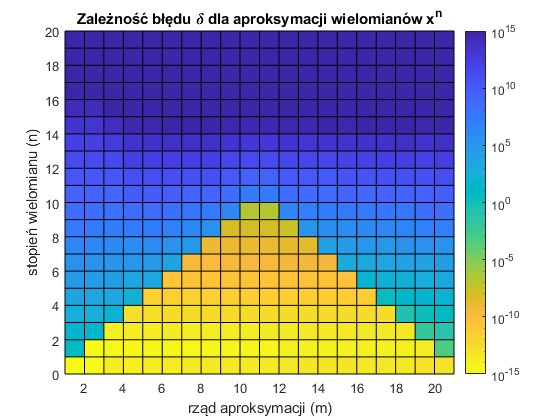
\includegraphics[width=1.05\linewidth]{figure1.jpg}
  \caption{Zastosowanie kwadratury rzędu $r = 20$}
  \label{fig:sub1}
\end{subfigure}%
\begin{subfigure}{.5\textwidth}
  \centering
  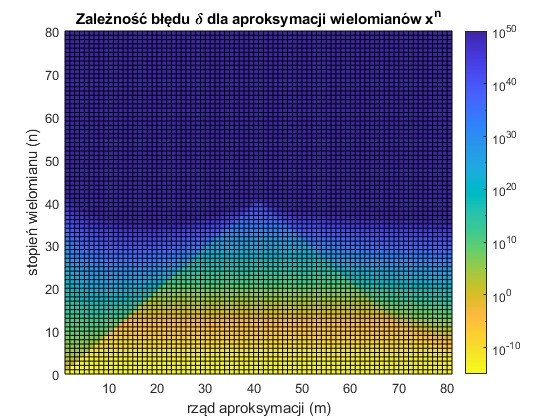
\includegraphics[width=1.05\linewidth]{figure2.jpg}
  \caption{Zastosowanie kwadratury rzędu $r = 80$}
  \label{fig:sub2}
\end{subfigure}
\caption{Błąd średniokwadratowy aproksymacji wielomianów postaci $x^n$, w zależności od rzędu aproksymacji $m$ oraz stopnia wielomianu $n$. Tablicowanie wartości funkcji i jej przybliżeń w 200 punktach z przedziału $[0,1].$}
\label{fig:test}
\end{figure}
\end{document}
